\documentclass[a4paper,10pt]{exam}
\usepackage{graphicx}
\usepackage[document]{ragged2e}
 \usepackage[margin=1in]{geometry}
\usepackage{circuitikz}
\pagestyle{empty}
\usepackage{tikz}
\usepackage{multirow}
\usepackage{float}
\usepackage{amsmath}
\usepackage{multicol}
\usepackage{array}
\usepackage{enumitem}
\usepackage{setspace}
\usepackage{amssymb}

\usepackage{cite}
\usepackage{graphicx}
\usepackage{amsmath,amssymb,amsfonts,amsthm}
\usepackage{algorithmic}
\usepackage{graphicx}
\usepackage{textcomp}
\usepackage{xcolor}
\usepackage{txfonts}
\usepackage{listings}
\usepackage{enumitem}
\usepackage{mathtools}
\usepackage{gensymb}
\usepackage{comment}
\usepackage[breaklinks=true]{hyperref}
\usepackage{tkz-euclide} 
\usepackage{listings}
\usepackage{gvv}                                        
%\def\inputGnumericTable{}                                 
\usetikzlibrary{arrows.meta, positioning}
\usepackage{xparse}
\usepackage{color}                                            
\usepackage{array}                                            
\usepackage{longtable}                                       
\usepackage{calc}                                             
\usepackage{multirow}
\usepackage{multicol}
\usepackage{hhline}                                           
\usepackage{ifthen}                                           
\usepackage{lscape}
\usepackage{tabularx}
\usepackage{array}
\usepackage{float}
\newtheorem{theorem}{Theorem}[section]
\newtheorem{problem}{Problem}
\newtheorem{proposition}{Proposition}[section]
\newtheorem{lemma}{Lemma}[section]
\newtheorem{corollary}[theorem]{Corollary}
\newtheorem{example}{Example}[section]
\newtheorem{definition}[problem]{Definition}
\newcommand{\BEQA}{\begin{eqnarray}}
\newcommand{\EEQA}{\end{eqnarray}}
\usepackage{float}
%\newcommand{\define}{\stackrel{\triangle}{=}}
\theoremstyle{remark}
\usepackage{circuitikz}
\usepackage{tikz}
\usepackage{ragged2e}
\begin{document}

\begin{center}
    \LARGE \textbf{GATE 2014 Examination} \\[2mm]
    \Large \textbf{CY: Chemistry}
\end{center}


\raggedright{{Duration:} \textbf{180 minutes} }\hfill Maximum Marks: \textbf{100}


\vspace{3mm}
\textbf{Read the following instructions carefully.}

\begin{enumerate}
    \item To login, enter your Registration Number and password provided to you. Kindly go through the various symbols used in the test and understand their meaning before you start the examination.
    \item Once you login and after the start of the examination, you can view all the questions in the question paper, by clicking on the \textbf{View All Questions} button in the screen.
    \item This question paper consists of \textbf{2 sections}, General Aptitude (GA) for \textbf{15 marks} and the subject specific GATE paper for \textbf{85 marks}. Both these sections are compulsory.\\
    The GA section consists of 10 questions. Question numbers 1 to 5 are of 1-mark each, while question numbers 6 to 10 are of 2-mark each.\\
    The subject specific GATE paper section consists of 55 questions, out of which question numbers 1 to 25 are of 1-mark each, while question numbers 26 to 55 are of 2-mark each.
    \item Depending upon the GATE paper, there may be useful common data that may be required for answering the questions. If the paper has such useful data, the same can be viewed by clicking on the \textbf{Useful Common Data} button that appears at the top, right hand side of the screen.
    \item The computer allotted to you at the examination center runs specialized software that permits only one answer to be selected for multiple-choice questions using a mouse and to enter a suitable number for the numerical answer type questions using the virtual keyboard and mouse.
    \item Your answers shall be updated and saved on a server periodically and also at the end of the examination. The examination will \textbf{stop automatically} at the end of \textbf{180 minutes}.
    \item In each paper a candidate can answer a total of 65 questions carrying 100 marks.
    \item The question paper may consist of questions of \textbf{multiple choice type (MCQ)} and \textbf{numerical answer type.}
    \item Multiple choice type questions will have four choices against A, B, C, D, out of which only \textbf{ONE} is the correct answer. The candidate has to choose the correct answer by clicking on the bubble $(\bigcirc)$ placed before the choice.
    \item For numerical answer type questions, each question will have a numerical answer and there will not be any choices. For these questions, \textbf{the answer should be entered} using the virtual keyboard that appears on the monitor and the mouse.
    \item All questions that are not attempted will result in zero marks. However, wrong answers for multiple choice type questions (MCQ) will result in \textbf{NEGATIVE} marks. For all MCQ questions a wrong answer will result in deduction of $\frac{1}{3}$ marks for a 1-mark question and $\frac{2}{3}$ marks for a 2-mark question.
    \item There is \textbf{NO NEGATIVE MARKING} for questions of \textbf{NUMERICAL ANSWER TYPE}.
    \item Non-programmable type Calculator is allowed. Charts, graph sheets, and mathematical tables are NOT allowed in the Examination Hall. You must use the Scribble Pad provided to you at the examination centre for all your rough work. The Scribble Pad has to be returned at the end of the examination.
\end{enumerate}

\vspace{6mm}
\textbf{Declaration by the candidate:}

\noindent I have read and understood all the above instructions. I have also read and understood clearly the instructions given on the admit card and shall follow them strictly. I also understand that in case I am found to violate the code of conduct for the examination, my candidature will be cancelled and I may also be debarred from appearing in future GATE examinations.
\newpage
\textbf{GATE 2014}\hspace{1in} \textbf{SET-1}\hfill \textbf{General Aptitude - GA}\\
\noindent\rule{\linewidth}{0.4pt}
\textbf{Q.1 - Q.5 carry one mark each.}

\begin{enumerate}
    \item A student is required to demonstrate a high level of \emph{comprehension} of the subject, especially in the social sciences.\\
    The word closest in meaning to \emph{comprehension} is\hfill{(GATE CY 2014)}

    \begin{multicols}{4}
    \begin{enumerate}
        \item understanding
        \item meaning
        \item concentration
        \item stability
    \end{enumerate}
    \end{multicols}

    \item Choose the most appropriate word from the options given below to complete the following sentence.\\
    One of his biggest \rule{1.5cm}{0.15mm} was his ability to forgive.\hfill{(GATE CY 2014)}

    \begin{multicols}{4}
    \begin{enumerate}
        \item vice
        \item virtues
        \item choices
        \item strength
    \end{enumerate}
    \end{multicols}

    \item Rajan was not happy that Sajan decided to do the project on his own. On observing his unhappiness, Sajan explained to Rajan that he preferred to work independently.\\
    Which one of the statements below is logically valid and can be inferred from the above sentences?\hfill{(GATE CY 2014)}

    \begin{enumerate}
        \item Rajan has decided to work only in a group.
        \item Rajan and Sajan were formed into a group against their wishes.
        \item Sajan had decided to give in to Rajan's request to work with him.
        \item Rajan had believed that Sajan and he would be working together.
    \end{enumerate}

    \item If $y=5x^2+3$, then the tangent at $x=0$, $y=3$\hfill{(GATE CY 2014)}
    \begin{multicols}{2}
    \begin{enumerate}
        \item passes through $x = 0$, $y = 0$
        \item has a slope of $+1$
        \item is parallel to the $x$-axis
        \item has a slope of $-1$
    \end{enumerate}
    \end{multicols}

    \item A foundry has a fixed daily cost of Rs 50,000 whenever it operates and a variable cost of Rs 800Q, where $Q$ is the daily production in tonnes. What is the cost of production in Rs per tonne for a daily production of 100 tonnes?\hfill{(GATE CY 2014)}


\vspace{1em}
\textbf{Q.6 -- Q. 10 carry two marks each.}
\vspace{1em}

    \item Find the odd one in the following group: ALRVX, EPVZB, ITZDF, OYEIK\hfill{(GATE CY 2014)}

    \begin{multicols}{4}
    \begin{enumerate}
        \item ALRVX
        \item EPVZB
        \item ITZDF
        \item OYEIK
    \end{enumerate}
    \end{multicols}

    \item Anuj, Bhola, Chandan, Dilip, Eswar and Faisal live on different floors in a six-storeyed building (the ground floor is numbered 1, the floor above it 2, and so on). Anuj lives on an even-numbered floor. Bhola does not live on an odd numbered floor. Chandan does not live on any of the floors below Faisal’s floor. Dilip does not live on floor number 2. Eswar does not live on a floor immediately above or immediately below Bhola. Faisal lives three floors above Dilip. Which of the following floor-person combinations is correct?\hfill{(GATE CY 2014)}

    \begin{center}
    \begin{tabular}{|c|c|c|c|c|c|c|}
      \hline
        & Anuj & Bhola & Chandan & Dilip & Eswar & Faisal \\
      \hline
      (A) & 2 & 6 & 1 & 3 & 4 & 5 \\
      (B) & 2 & 6 & 5 & 1 & 3 & 4 \\
      (C) & 4 & 2 & 6 & 3 & 1 & 5 \\
      (D) & 2 & 4 & 6 & 1 & 3 & 5 \\
      \hline
    \end{tabular}
    \end{center}
    
\vfill
\noindent\rule{\linewidth}{0.4pt}
GA \hfill 1/2
\newpage
\textbf{GATE 2014}\hspace{1in} \textbf{SET-1}\hfill \textbf{General Aptitude - GA}\\
\noindent\rule{\linewidth}{0.4pt}

\item The smallest angle of a triangle is equal to two thirds of the smallest angle of a quadrilateral. The ratio between the angles of the quadrilateral is $3:4:5:6$. The largest angle of the triangle is twice its smallest angle. What is the sum, in degrees, of the second largest angle of the triangle and the largest angle of the quadrilateral?\hfill{(GATE CY 2014)}

    \item One percent of the people of country X are taller than 6 ft. Two percent of the people of country Y are taller than 6 ft. There are thrice as many people in country X as in country Y. Taking both countries together, what is the percentage of people taller than 6 ft?\hfill{(GATE CY 2014)}
    \begin{multicols}{4}
    \begin{enumerate}
        \item 3.0
        \item 2.5
        \item 1.5
        \item 1.25
    \end{enumerate}
    \end{multicols}

    \item The monthly rainfall chart based on 50 years of rainfall in Agra is shown in the following figure. Which of the following are true? ($k$ percentile is the value such that $k$ percent of the data fall below that value)

\begin{figure}[H]
    \centering
    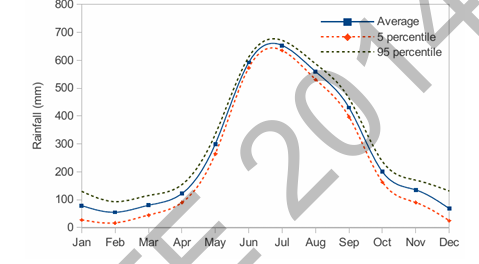
\includegraphics[width=0.7\columnwidth]{figs/Q 10.png}
    \caption{}
    \label{fig:placeholder}
\end{figure}
    
    (i) On average, it rains more in July than in December \\
    (ii) Every year, the amount of rainfall in August is more than that in January \\
    (iii) July rainfall can be estimated with better confidence than February rainfall \\
    (iv) In August, there is at least 500 mm of rainfall\hfill{(GATE CY 2014)}

    \begin{multicols}{2}
    \begin{enumerate}
        \item (i) and (ii)
        \item (i) and (iii)
        \item (ii) and (iii)
        \item (iii) and (iv)
    \end{enumerate}
    \end{multicols}
\end{enumerate}
\vfill
\noindent\rule{\linewidth}{0.4pt}
GA \hfill 2/2
\newpage
GATE 2014\hfill CHEMISTRY - CY\\
\noindent\rule{\linewidth}{0.4pt}
\begin{center}
    USEFUL DATA - CY CHEMISTRY
\end{center}
\begin{center}
    \textbf{COMMON DATA}
\end{center}
$\begin{array}{ll}
\text{Gas constant} \qquad & : \quad 8.314~\mathrm{J~K^{-1}~mol^{-1}} \\
                           & : \quad 0.083~\mathrm{L~bar~K^{-1}~mol^{-1}} \\
\text{Faraday constant}    & : \quad 96500~\mathrm{C~mol^{-1}} \\
\text{2.303RT/F at 300~K}  & : \quad 0.06~\mathrm{V} \\
N_\text{A}                 & : \quad 6.02 \times 10^{23} \\
\text{Atomic numbers}      & : \quad \text{B = 5, N = 7, Mg = 12, S = 16, Ti = 22, V = 23, Cr = 24, Mn = 25} \\
                           & \quad  \text{Fe = 26, Co = 27, Ni = 28, Cu = 29, Rh = 45, Ta = 73}
\end{array}
$
\vfill
\noindent\rule{\linewidth}{0.4pt}
CY \hfill 1 /11
\newpage
GATE 2014\hfill CHEMISTRY - CY\\
\noindent\rule{\linewidth}{0.4pt}
\textbf{Q.1 - Q.25 carry one mark each.}
\begin{enumerate}
\item The maximum non-$PV$ work that a system can perform at constant $P$ is\hfill{(GATE CY 2014)}
    \begin{multicols}{4}
    \begin{enumerate}
        \item $\Delta H$
        \item $\Delta G$
        \item $\Delta S$
        \item $\Delta A$
    \end{enumerate}
    \end{multicols}

    \item Consider the reaction: \\
    \hspace*{1cm} A + B $\rightleftharpoons$ C \\
    The unit of the thermodynamic equilibrium constant for the reaction is\hfill{(GATE CY 2014)}
    \begin{multicols}{4}
    \begin{enumerate} 
        \item mol L$^{-1}$
        \item L mol$^{-1}$
        \item mol$^{2}$ L$^{-2}$
        \item dimensionless
    \end{enumerate}
    \end{multicols}

    \item The number of IR active vibrational normal modes of $CO_2$ is \underline{\hspace{2cm}}\hfill{(GATE CY 2014)}

    \item The number of C$_2$ axes in CCl$_4$ is \underline{\hspace{2cm}}\hfill{(GATE CY 2014)}

    \item The value of the magnetic quantum number of a $p_x$ orbital is\hfill{(GATE CY 2014)}
    \begin{multicols}{4}
    \begin{enumerate} 
        \item $-1$
        \item $0$
        \item $+1$
        \item undefined
    \end{enumerate}
    \end{multicols}

    \item The molecular partition function for a system in which the energy levels are equispaced by $\epsilon$, is\hfill{(GATE CY 2014)}
    \begin{multicols}{4}
    \begin{enumerate} 
        \item $\dfrac{1}{1 + e^{\beta\epsilon}}$
        \item $\dfrac{1}{1 - e^{\beta\epsilon}}$
        \item $\dfrac{1}{1 + e^{-\beta\epsilon}}$
        \item $\dfrac{1}{1 - e^{-\beta\epsilon}}$
    \end{enumerate}
    \end{multicols}

    \item A monoatomic gas, $X$, adsorbed on a surface, follows Langmuir adsorption isotherm. A plot of the fraction of surface coverage, $\theta$, against the concentration of the gas $[X]$,  for \textbf{VERY LOW} concentration of the gas, is described by the equation\hfill{(GATE CY 2014)}
    \begin{multicols}{2}
    \begin{enumerate} 
        \item $\theta = K [X]$
        \item $1 - \theta = \dfrac{1}{K [X]}$
        \item $\theta = K^{1/2} [X]^{1/2}$
        \item $\theta = \dfrac{K[X]}{1-K[X]}$
    \end{enumerate}
    \end{multicols}

    \item At a given temperature and pressure, the ratio of the average speed of hydrogen gas to that of helium gas is approximately \underline{\hspace{2cm}}\hfill{(GATE CY 2014)}

    \item An example of \textit{nido}-borane from the following is\hfill{(GATE CY 2014)}
    \begin{multicols}{4}
    \begin{enumerate} 
        \item B$_4$H$_{10}$
        \item B$_5$H$_{10}$
        \item B$_4$H$_{12}$
        \item B$_5$H$_{14}$
    \end{enumerate}
    \end{multicols}

    \item The geometries of Ni(CO)$_4$ and [NiCl$_4$]$^{2-}$, respectively, are\hfill{(GATE CY 2014)}
    \begin{multicols}{2}
    \begin{enumerate} 
        \item tetrahedral and square planar
        \item square planar and tetrahedral
        \item tetrahedral and tetrahedral
        \item square planar and square planar
    \end{enumerate}
    \end{multicols}

    \item The number of S–S bonds in H$_2$S$_2$O$_6$ is \underline{\hspace{2cm}}\hfill{(GATE CY 2014)}

    \item In atomic absorption spectroscopy, the atomization process utilizes\hfill{(GATE CY 2014)}
    \begin{multicols}{4}
    \begin{enumerate} 
        \item flame
        \item electric field
        \item magnetic field
        \item electron beam
    \end{enumerate}
    \end{multicols}

    \item At room temperature, the number of singlet resonances observed in the $^{1}$H NMR spectrum of Me$_3$CC(O)NMn$_2$ (N,N-dimethyl pivalamide) is \underline{\hspace{2cm}}\hfill{(GATE CY 2014)}
\vfill
\noindent\rule{\linewidth}{0.4pt}
CY \hfill 2 /11
\newpage
GATE 2014\hfill CHEMISTRY - CY\\
\noindent\rule{\linewidth}{0.4pt}

\item Amongst the following, the metal that does \textbf{NOT} form homoleptic polynuclear metal carbonyl is\hfill{(GATE CY 2014)}
    \begin{multicols}{4}
    \begin{enumerate} 
        \item Mn
        \item Fe
        \item Cr
        \item Co
    \end{enumerate}
    \end{multicols}

    \item The reaction of [Cp$_2$TaMe$_2$]I (Cp = C$_5$H$_5^{-}$) with NaOMe yields\hfill{(GATE CY 2014)}
    \begin{multicols}{2}
    \begin{enumerate} 
        \item (Cp$_2$Ta(OMe)$_2$)I
        \item (Cp$_2$Ta(Me)OMe)I
        \item Cp$_2$Ta(Me)$=$CH$_2$
        \item Cp$_2$Ta(OMe)$=$CH$_2$
    \end{enumerate}
    \end{multicols}

    \item The complexes [Co(H$_2$O)$_4$Cl$_2$]NO$_2$ and [Co(H$_2$O)$_4$Cl(NO$_2$)]Cl are\hfill{(GATE CY 2014)}
    \begin{multicols}{2}
    \begin{enumerate} 
        \item linkage isomers
        \item positional isomers
        \item ionization isomers
        \item optical isomers
    \end{enumerate}
    \end{multicols}

    \item The major product of the following reaction is\hfill{(GATE CY 2014)}
    \begin{figure}[H]
        \centering
        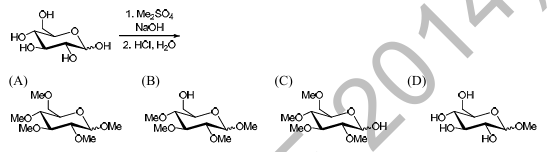
\includegraphics[width=0.9\columnwidth]{figs/Q 17.png}
        \caption{}
        \label{fig:placeholder}
    \end{figure}
\item Amongst the following, the struture of guanosine is\hfill{(GATE CY 2014)}
\begin{figure}[H]
    \centering
    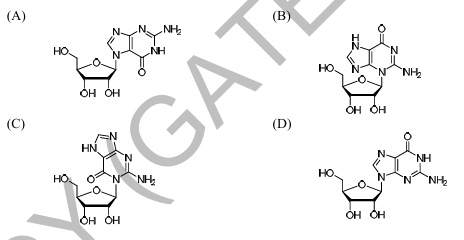
\includegraphics[width=0.8\columnwidth]{figs/Q 18.png}
    \caption{}
    \label{fig:placeholder}
\end{figure}
\vfill
\noindent\rule{\linewidth}{0.4pt}
CY \hfill 3 /11
\newpage
GATE 2014\hfill CHEMISTRY - CY\\
\noindent\rule{\linewidth}{0.4pt}
\item The correct order of IR stretching frequency of the C=C in the following olefins is\hfill{(GATE CY 2014)}
\begin{figure}[H]
    \centering
    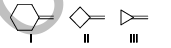
\includegraphics[width=0.4\columnwidth]{figs/Q 19.png}
    \caption{}
    \label{fig:placeholder}
\end{figure}
 \begin{multicols}{4}
    \begin{enumerate} 
        \item I      $>$ II      $>$ III
        \item II      $>$ III      $>$ I 
        \item III      $>$ II      $>$ I
        \item III      $>$ I      $>$ II
    \end{enumerate}
    \end{multicols}
\item The correct order of the rate of solvolysis for the following chlorides in acetic acid is\hfill{(GATE CY 2014)}
\begin{figure}[h]
    \centering
    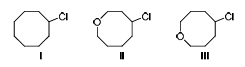
\includegraphics[width=0.5\columnwidth]{figs/Q 20.png}
    \caption{}
    \label{fig:placeholder}
\end{figure}
\begin{multicols}{4}
    \begin{enumerate} 
        \item II      $>$ I      $>$ III
        \item III      $>$ II      $>$ I 
        \item III      $>$ I      $>$ II
        \item I      $>$ III      $>$ II
    \end{enumerate}
    \end{multicols}
\item Formation of the product in the following photochemical reaction involves\hfill{(GATE CY 2014)}
\begin{figure}[H]
    \centering
    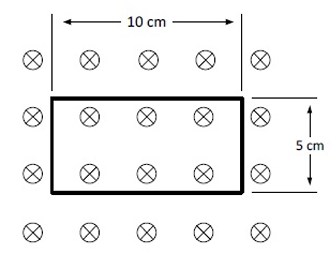
\includegraphics[width=0.5\columnwidth]{figs/Q 21.png}
    \caption{}
    \label{fig:placeholder}
\end{figure}

\begin{multicols}{4}
    \begin{enumerate} 
        \item  di-$\pi$-methane rearrangement 
        \item Paterno-Buchi reaction 
        \item  [2,3]-sigmatropic rearrangement
        \item Norrish type I reaction
    \end{enumerate}
    \end{multicols}
\item The correct order of stability for the following conformations of cyclohexane is\hfill{(GATE CY 2014)}
\begin{figure}[H]
    \centering
    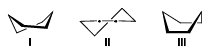
\includegraphics[width=0.5\columnwidth]{figs/Q 22.png}
    \caption{}
    \label{fig:placeholder}
\end{figure}
\begin{multicols}{4}
    \begin{enumerate} 
        \item I      $>$ II      $>$ III
        \item I      $>$ III      $>$ II 
        \item II      $>$ I      $>$ III
        \item III     $>$ I      $>$ II
    \end{enumerate}
    \end{multicols}
    
\vfill
\noindent\rule{\linewidth}{0.4pt}
CY \hfill 4 /11
\newpage
GATE 2014\hfill CHEMISTRY - CY\\
\noindent\rule{\linewidth}{0.4pt}
 
\item The major product formed in the following reaction is\hfill{(GATE CY 2014)}
\begin{figure}[H]
    \centering
    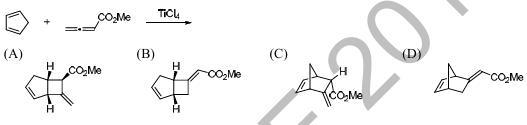
\includegraphics[width=1\columnwidth]{figs/Q 23.png}
    \caption{}
    \label{fig:placeholder}
\end{figure}
\item The overall yield (in \%) for the following reaction sequence is \rule{1.5cm}{0.15mm}\hfill{(GATE CY 2014)}
\begin{figure}[H]
    \centering
    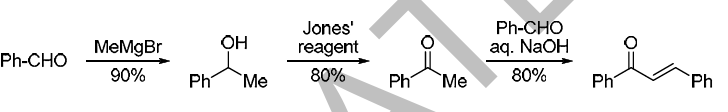
\includegraphics[width=0.7\columnwidth]{figs/Q 24.png}
    \caption{}
    \label{fig:placeholder}
\end{figure}
\item The most suitable reagent combination to effect the following conversion is\hfill{(GATE CY 2014)}
\begin{figure}[H]
    \centering
    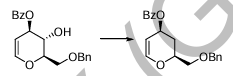
\includegraphics[width=0.5\columnwidth]{figs/Q 25.png}
    \caption{}
    \label{fig:placeholder}
\end{figure}
\begin{enumerate}
    \item i. NaH, CS$_2$, then MeI; \quad ii. Bu$_3$SnH, AIBN, C$_6$H$_6$, reflux

    \item i. I$_2$, PPh$_3$, imidazole; \quad ii. H$_2$, 10\% Pd-C, AcOH, high pressure

    \item i. Me$_3$SiCl, pyridine, DMAP; \quad ii. Bu$_3$SnH, AIBN, C$_6$H$_6$, reflux

    \item i. MsCl, pyridine, DMAP; \quad ii. LiAlH$_4$, THF, reflux
\end{enumerate}
\textbf{Q.26 - Q.55 carry two marks each.}

\item $\psi = N\, r (6 - Z\, r)\, e^{-Z r/3} \cos \theta$ , is a proposed hydrogenic wavefunction, where $Z=$ Atomic number, $r=$ radial distance from the nucleus, $\theta =$ azimuthal angle, $N$ is a constant. The \textbf{INCORRECT} statement about $\psi$ is\hfill{(GATE CY 2014)}
\begin{enumerate}
    \item $\psi = 0$ in the $xy$-plane
    \item two radial nodes are present in $\psi$
    \item one angular node is present in $\psi$
    \item the size of the orbital decreases with increase in atomic number
\end{enumerate}
\vfill
\noindent\rule{\linewidth}{0.4pt}
CY \hfill 5 /11
\newpage
GATE 2014\hfill CHEMISTRY - CY\\
\noindent\rule{\linewidth}{0.4pt}
\item The van der Waals constants $a$ and $b$ of CO$_2$ are 3.64~L$^2$~bar~mol$^{-2}$ and 0.04~L~mol$^{-1}$, respectively. The value of $R$ is 0.083~bar~dm$^3$~mol$^{-1}$~K$^{-1}$. If one mole of CO$_2$ is confined to a volume of 0.15~L at 300~K, then the pressure (in bar) exerted by the gas, is \underline{\hspace{2cm}}\hfill{(GATE CY 2014)}

\item A plot of osmotic pressure against concentration (g~L$^{-1}$) of a polymer is constructed. The slope of the plot\hfill{(GATE CY 2014)}
\begin{enumerate}
    \item increases with increase in temperature
    \item increases with increase in molar mass of the polymer
    \item decreases with decrease in concentration of the polymer
    \item decreases with increase in temperature
\end{enumerate}

\item A platinum electrode is immersed in a solution containing 0.1~M Fe$^{2+}$ and 0.1~M Fe$^{3+}$. Its potential is found to be 0.77~V against SHE. Under standard conditions and considering activity coefficients to be equal to unity, the potential of the electrode, when the concentration of Fe$^{3+}$ is increased to 1~M, is \underline{\hspace{2cm}}\hfill{(GATE CY 2014)}

\item Molybdenum crystallizes in a \textit{bcc} structure with unit cell dimensions of 0.314~nm. Considering the atomic mass of molybdenum to be 96, its density (in kg~m$^{-3}$) is \underline{\hspace{2cm}}\hfill{(GATE CY 2014)}

\item The ratio of molecules distributed between two states is $9.22 \times 10^6$ at 300~K. The difference in energy (in kJ~mol$^{-1}$) of the two states is \underline{\hspace{2cm}}\hfill{(GATE CY 2014)}

\item A Carnot engine operates at 55\% efficiency. If the temperature of reject steam is 105~$^\circ$C, then the absolute temperature of input steam is \underline{\hspace{2cm}}\hfill{(GATE CY 2014)}

\item Of the following plots, the correct representation of chemical potential ($\mu$) against absolute temperature ($T$) for a pure substance is ($s,~l$ and $g$ denote solid, liquid and gas phases, respectively) \hfill{(GATE CY 2014)}
\begin{figure}[H]
    \centering
    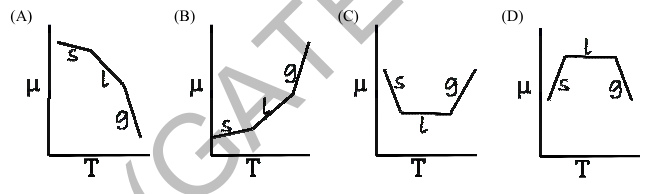
\includegraphics[width=0.9\columnwidth]{figs/Q 33.png}
    \caption{}
    \label{fig:placeholder}
\end{figure}
\item The enthalpy of fusion of ice at 273 K is 6.01 kJ mol$^{-1}$ and the enthalpy of vaporization of water at 273 K is 44.83 kJ mol$^{-1}$. The enthalpy of sublimation (in kJ mol$^{-1}$) of ice at 273 K, is \underline{\hspace{2cm}}\hfill{(GATE CY 2014)}
\item Suppose $\psi_1$ and $\psi_2$ are two hybrid orbitals:\\
$
\psi_1=0.12\,\psi_{3s}+0.63\,\psi_{3p_x}+0.77\,\psi_{3p_y}
$
and
$
\psi_2=0.12\,\psi_{3s}-0.63\,\psi_{3p_x}-0.77\,\psi_{3p_y}
$
The angle (in degrees) between them is \underline{\hspace{2cm}}\hfill{(GATE CY 2014)}
\item BCl$_3$ and NH$_4$Cl were heated at 140$^\circ$C to give compound \textbf{X}, which when treated with NaBH$_4$ gave another compound \textbf{Y}. Compounds \textbf{X} and \textbf{Y} are\hfill{(GATE CY 2014)}
\begin{enumerate}
    \item X = B$_3$N$_3$H$_3$Cl$_3$ and Y = B$_3$N$_3$H$_6$
    \item X = B$_3$N$_3$H$_6$Cl$_3$ and Y = B$_3$N$_3$H$_6$
    \item X = B$_3$N$_3$H$_3$Cl$_{12}$ and Y = B$_3$N$_3$H$_{12}$
    \item X = B$_3$N$_3$Cl$_6$ and Y = B$_3$N$_3$H$_6$
\end{enumerate}
\vfill
\noindent\rule{\linewidth}{0.4pt}
CY \hfill 6 /11
\newpage
GATE 2014\hfill CHEMISTRY - CY\\
\noindent\rule{\linewidth}{0.4pt}
\item The number of microstates in term $^1$G is \underline{\hspace{2cm}}\hfill{(GATE CY 2014)}
\item The set of protons (underlined) in CH$_3$CH$_2$CH$_2$OCH$_3$ that would exhibit different splitting patterns in high (500 MHz) and low (60 MHz) field $^1$H NMR, is\hfill{(GATE CY 2014)}
\begin{enumerate}
    \item \underline{CH}$_3$CH$_2$CH$_2$OCH$_3$
    \item CH$_3$\underline{CH}$_2$CH$_2$OCH$_3$
    \item CH$_3$CH$_2$\underline{CH}$_2$OCH$_3$
    \item CH$_3$CH$_2$CH$_2$OCH$_3$
\end{enumerate}


\item Amongst the following, the complex ion that would show strong Jahn-Teller distortion is\hfill{(GATE CY 2014)}
\begin{multicols}{4}
\begin{enumerate}
    \item [Cr(H$_2$O)$_6$]$^{2+}$
    \item [Ti(H$_2$O)$_6$]$^{3+}$
    \item [Co(H$_2$O)$_6$]$^{2+}$
    \item [Fe(H$_2$O)$_6$]$^{2+}$
\end{enumerate}
\end{multicols} 

\item Amongst the following, the metal carbonyl species having the highest $\nu_{\mathrm{CO}}$ stretching frequency is\hfill{(GATE CY 2014)}
\begin{multicols}{4}
\begin{enumerate} 
    \item Mn(CO)$_6$$^{+}$
    \item Cr(CO)$_6$
    \item V(CO)$_6$$^{-}$
    \item Fe(CO)$_4$$^{2-}$
\end{enumerate}
\end{multicols}

\item The correct order of thermal stability for the given compounds is\hfill{(GATE CY 2014)}
\begin{enumerate} 
    \item TiMe$_4 >$ Ti(CH$_2$CMe$_3$)$_4 >$ TiEt$_4$
    \item TiEt$_4 >$ Ti(CH$_2$CMe$_3$)$_4 >$ TiMe$_4$
    \item TiMe$_4 >$ TiEt$_4 >$ Ti(CH$_2$CMe$_3$)$_4$
    \item Ti(CH$_2$CMe$_3$)$_4 >$ TiMe$_4 >$ TiEt$_4$
\end{enumerate}

\item
Amongst the following, the complex ion that is expected to show the highest magnetic moment at room temperature is\hfill{(GATE CY 2014)}
\begin{multicols}{4}
\begin{enumerate} 
    \item Ni(CN)$_4$$^{2-}$
    \item Fe(CN)$_6$$^{3-}$
    \item Cu(H$_2$O)$_6$$^{2+}$
    \item Co(CN)$_6$$^{3-}$
\end{enumerate}
\end{multicols} 

\item MnCr$_2$O$_4$ is\hfill{(GATE CY 2014)}
\begin{enumerate} 
    \item normal spinel with total CFSE of $-15.5$ Dq
    \item inverse spinel with total CFSE of $-15.5$ Dq
    \item normal spinel with total CFSE of $-24$ Dq
    \item inverse spinel with total CFSE of $-24$ Dq
\end{enumerate}
\item Mg$^{2+}$ is preferred in photosynthesis by chlorophyll because\hfill{(GATE CY 2014)}
\begin{enumerate} 
    \item it has strong spin-orbit coupling
    \item it has weak spin-orbit coupling
    \item it is a heavy metal
    \item it binds strongly with chlorophyll
\end{enumerate}
\vfill
\noindent\rule{\linewidth}{0.4pt}
CY \hfill 7 /11
\newpage
GATE 2014\hfill CHEMISTRY - CY\\
\noindent\rule{\linewidth}{0.4pt}
\item In Monsanto acetic acid process shown below, the role of HI is\hfill{(GATE CY 2014)}
\begin{figure}[H]
    \centering
    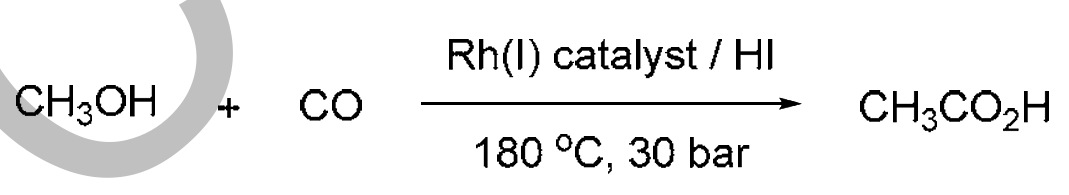
\includegraphics[width=0.5\columnwidth]{figs/Q 45.png}
    \caption{}
    \label{fig:placeholder}
\end{figure}

\begin{enumerate} 
    \item to convert CH$_3$OH to a stronger nucleophile (CH$_3$O$^{-}$)
    \item to reduce the Rh(I) catalyst to a Rh(0) species
    \item to reduce a Rh(III) active species to a Rh(I) species in the catalytic cycle
    \item to convert CH$_3$OH to CH$_3$I
\end{enumerate}
\item Formation of the ketone II from the diazoketone I involves \hfill{(GATE CY 2014)}

\begin{figure}[H]
    \centering
    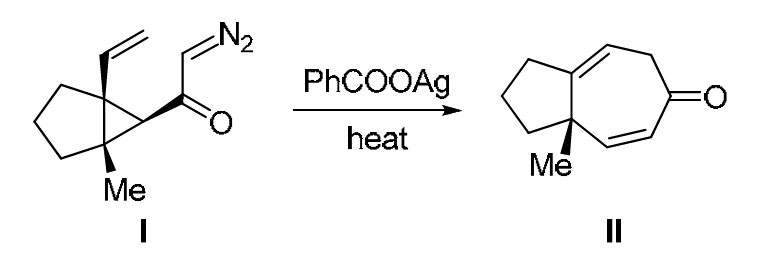
\includegraphics[width=0.4\columnwidth]{figs/Q 46.png}
    \caption{}
    \label{fig:placeholder}
\end{figure}

\begin{enumerate} 
    \item  generation of carbene and a [2,3]-sigmatropic rearrangement 
    \item  generation of carbene and an electrocyclic ring closing reaction 
    \item  generation of ketene and a [2+2] cycloaddition 
    \item generation of ketene and a [3,3]-sigmatropic rearrangement
\end{enumerate}
\item The major products X and Y formed in the following reaction sequence are \hfill{(GATE CY 2014)}
\begin{figure}[H]
    \centering
    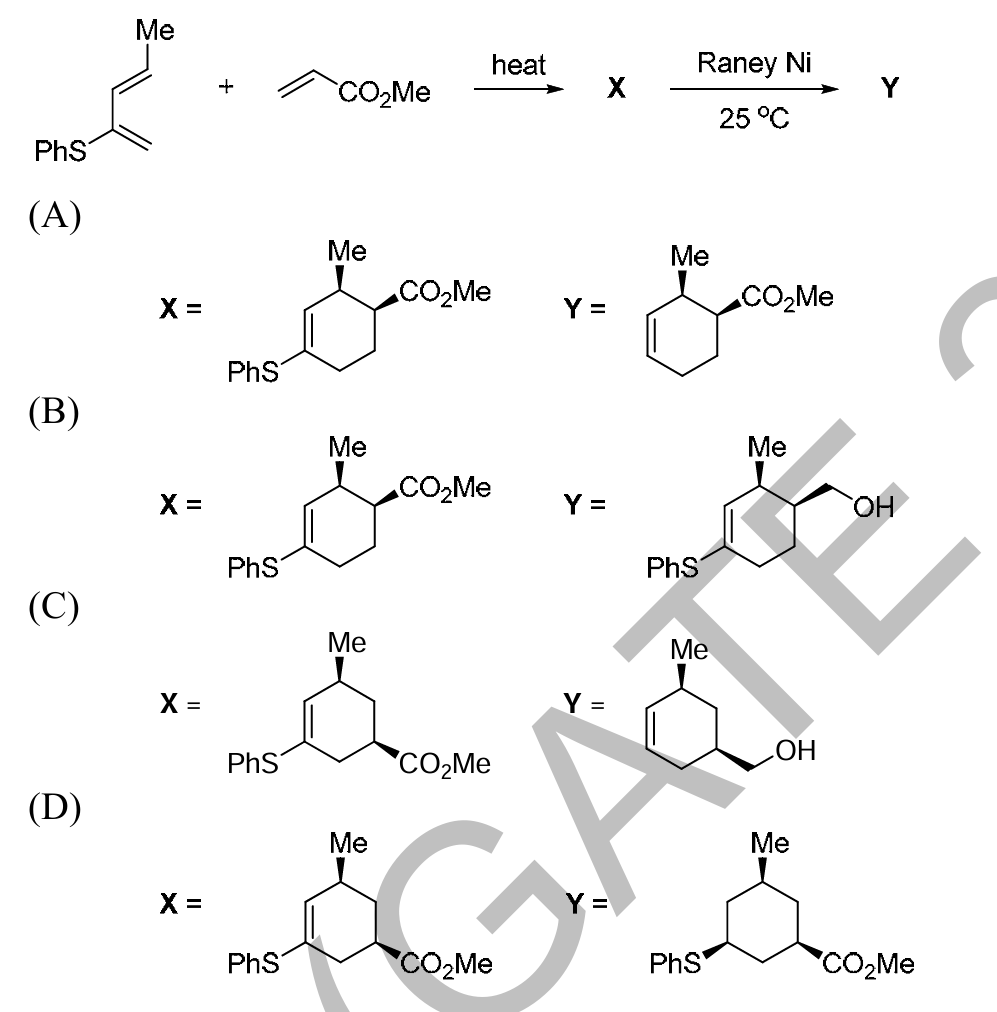
\includegraphics[width=0.5\columnwidth]{figs/Q 47.png}
    \caption{}
    \label{fig:placeholder}
\end{figure}
\vfill
\noindent\rule{\linewidth}{0.4pt}
CY \hfill 8 /11
\newpage
GATE 2014\hfill CHEMISTRY - CY\\
\noindent\rule{\linewidth}{0.4pt}

\item  The major products X and Y formed in the following reactions are \hfill{(GATE CY 2014)}

\begin{figure}[H]
    \centering
    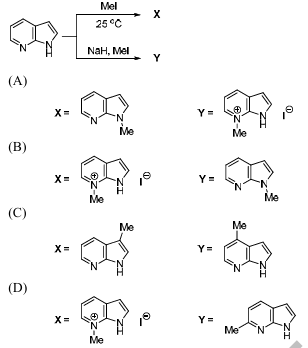
\includegraphics[width=0.5\columnwidth]{figs/Q 48.png}
    \caption{}
    \label{fig:placeholder}
\end{figure}

\item The major products X and Y formed in the following reaction sequence are \hfill{(GATE CY 2014)}
\begin{figure}[H]
    \centering
    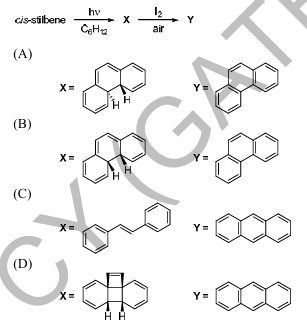
\includegraphics[width=0.5\columnwidth]{figs/Q 49.png}
    \caption{}
    \label{fig:placeholder}
\end{figure}
\vfill
\noindent\rule{\linewidth}{0.4pt}
CY \hfill 9 /11
\newpage
GATE 2014\hfill CHEMISTRY - CY\\
\noindent\rule{\linewidth}{0.4pt}

\item The product of the following reaction gave 6 line $^{13}$C NMR spectrum with peaks at $\delta$ 175, 52, 50, 
46, 37, 33 ppm. The structure of the product is\hfill{(GATE CY 2014)}
\begin{figure}[H]
    \centering
    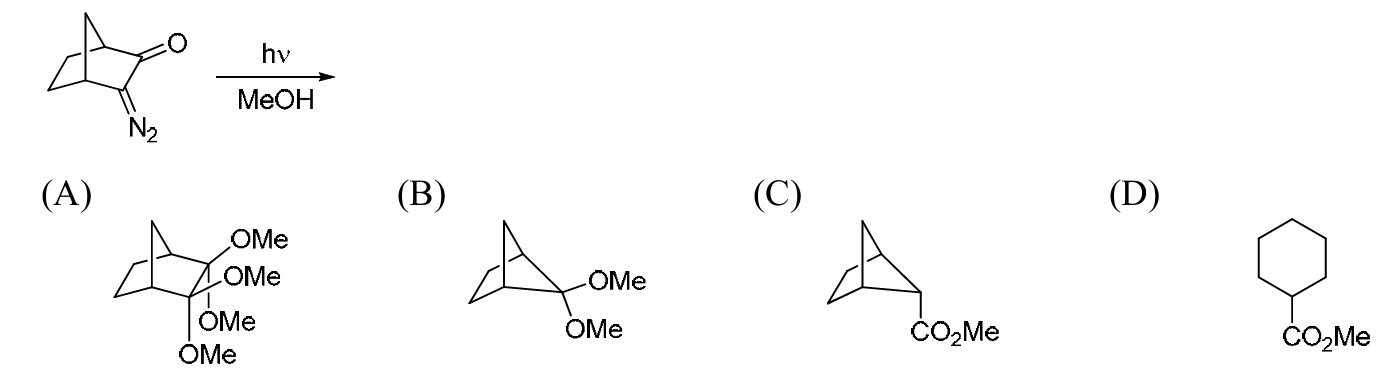
\includegraphics[width=0.8\columnwidth]{figs/Q 50.png}
    \caption{}
    \label{fig:placeholder}
\end{figure}
\item The major product formed in the following reaction is\hfill{(GATE CY 2014)}
\begin{figure}[H]
    \centering
    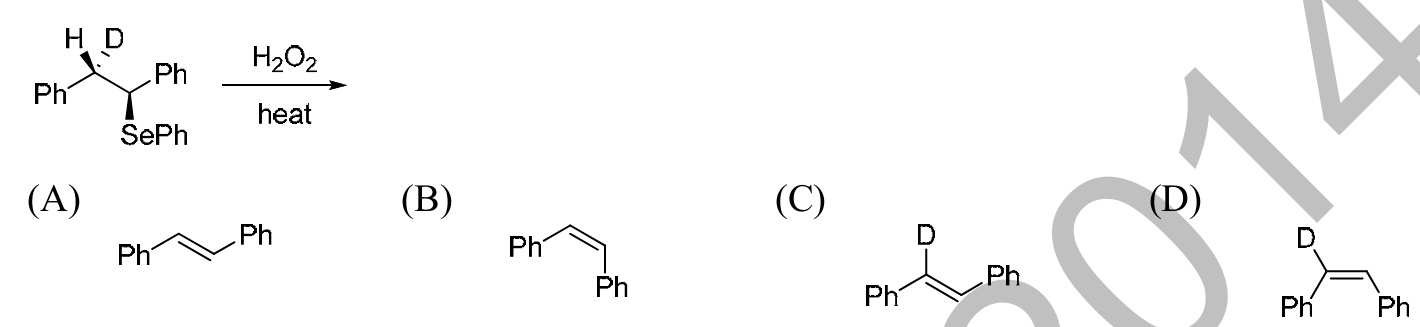
\includegraphics[width=0.8\columnwidth]{figs/Q 51.png}
    \caption{}
    \label{fig:placeholder}
\end{figure}

\item The major products X and Y formed in the following reaction sequence are\hfill{(GATE CY 2014)}
\begin{figure}[H]
    \centering
    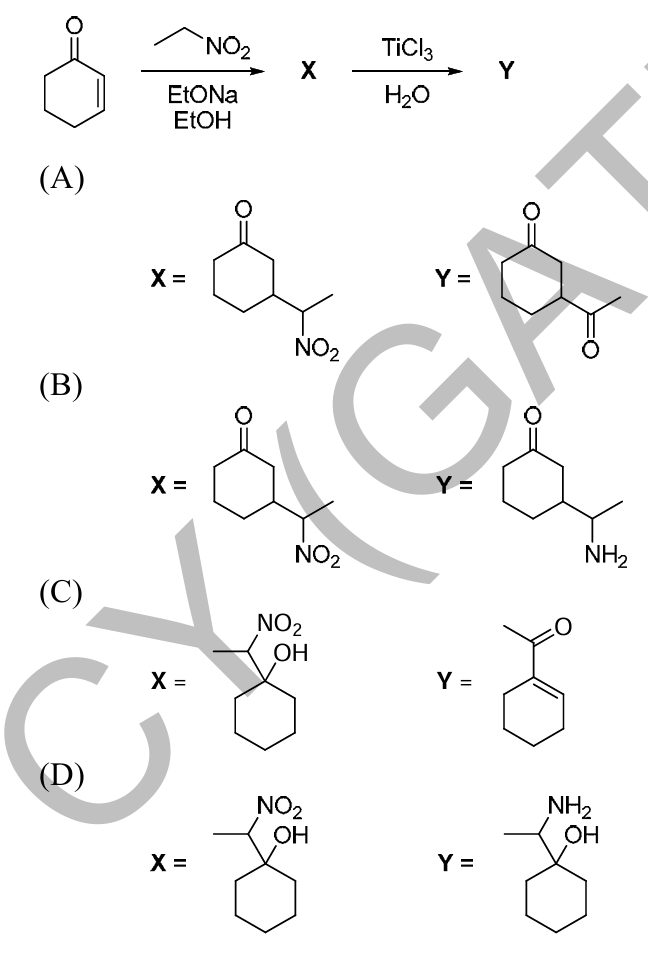
\includegraphics[width=0.4\columnwidth]{figs/Q 52.png}
    \caption{}
    \label{fig:placeholder}
\end{figure}
\vfill
\noindent\rule{\linewidth}{0.4pt}
CY \hfill 10 /11
\newpage
GATE 2014\hfill CHEMISTRY - CY\\
\noindent\rule{\linewidth}{0.4pt}
\item The major products X and Y formed in the following reaction sequence are\hfill{(GATE CY 2014)}
\begin{figure}[H]
    \centering
    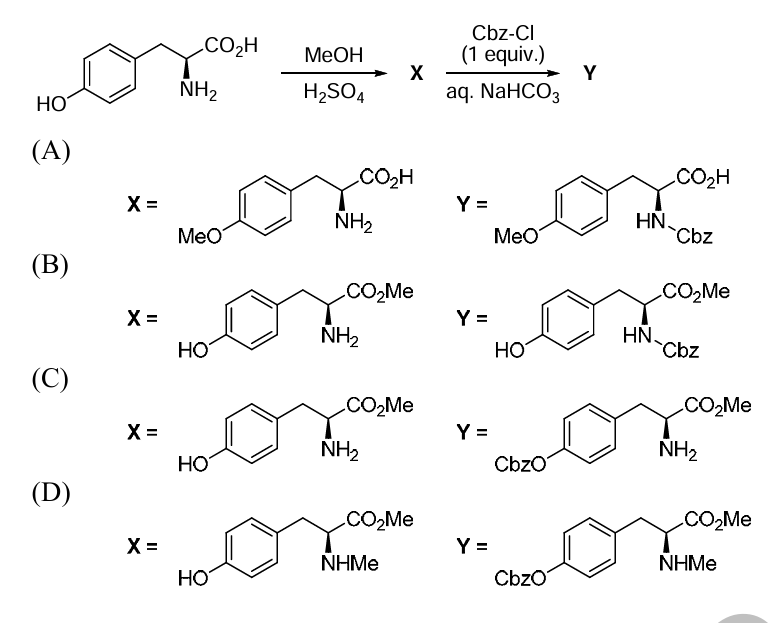
\includegraphics[width=0.5\columnwidth]{figs/Q 53.png}
    \caption{}
    \label{fig:placeholder}
\end{figure}
\item Given the fact that 1,3-butadiene has a UV absorption of 217 nm, the absorption wavelength (in 
nm) for the conjugated system shown below is \hfill{(GATE CY 2014)}
\begin{figure}[H]
    \centering
    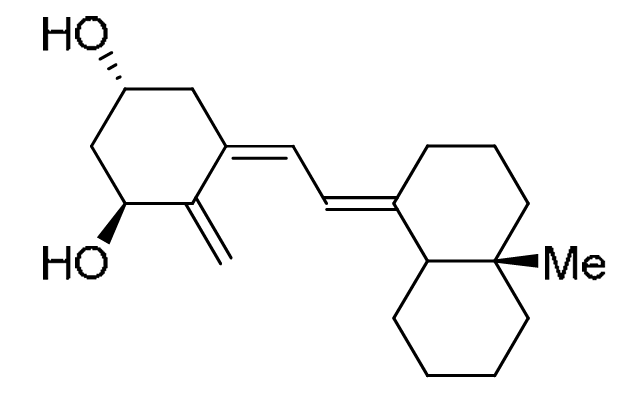
\includegraphics[width=0.4\linewidth]{figs/Q 54.png}
    \caption{}
    \label{fig:placeholder}
\end{figure}
(Use these absorption values for auxochromic groups: \\
alkyl: +5; exo-cyclic double bond: +5; every additional conjugated C=C: +30) 
\item The m/z value of the detectable fragment formed by McLafferty like rearrangement of the following 
compound in mass spectrometer is\hfill{(GATE CY 2014)}
\begin{figure}[H]
    \centering
    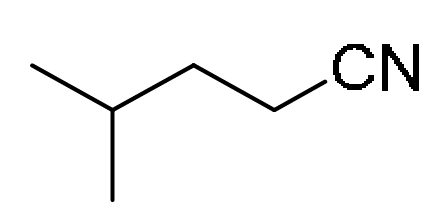
\includegraphics[width=0.3\columnwidth]{figs/Q 55.png}
    \caption{}
    \label{fig:placeholder}
\end{figure}
\begin{center}
    \textbf{END OF THE QUESTION PAPER }
\end{center}
\vfill
\noindent\rule{\linewidth}{0.4pt}
CY \hfill 11 /11
\newpage
\begin{center}
    \textbf{GATE 2014\\ Answer Keys for CY - Chemistry}
\end{center}
\noindent
\begin{minipage}{0.49\textwidth}
\begin{tabular}{|c|c|c|c|}
\hline
Section & Q. No. & Key / Range & Marks \\
\hline
GA & 1 & A & 1 \\
GA & 2 & B & 1 \\
GA & 3 & D & 1 \\
GA & 4 & C & 1 \\
GA & 5 & 1300 to 1300 & 1 \\
GA & 6 & D & 2 \\
GA & 7 & B & 2 \\
GA & 8 & 180 to 180 & 2 \\
GA & 9 & D & 2 \\
GA & 10 & B & 2 \\
CY & 1 & B & 1 \\
CY & 2 & D & 1 \\
CY & 3 & 3 to 3 & 1 \\
CY & 4 & 3 to 3 & 1 \\
CY & 5 & D & 1 \\
CY & 6 & D & 1 \\
CY & 7 & A & 1 \\
CY & 8 & 1.4 to 1.5 & 1 \\
CY & 9 & B & 1 \\
CY & 10 & C & 1 \\
CY & 11 & 4 to 4 & 1 \\
CY & 12 & A & 1 \\
CY & 13 & 3 to 3 & 1 \\
CY & 14 & C & 1 \\
CY & 15 & C & 1 \\
CY & 16 & C & 1 \\
CY & 17 & C & 1 \\
CY & 18 & D & 1 \\
CY & 19 & C & 1 \\
CY & 20 & B & 1 \\
CY & 21 & A & 1 \\
CY & 22 & B & 1 \\
CY & 23 & C & 1 \\
\hline
\end{tabular}
\end{minipage}
%
\hfill
%
\begin{minipage}{0.49\textwidth}
\begin{tabular}{|c|c|c|c|}
\hline
Section & Q. No. & Key / Range & Marks \\
\hline
CY & 24 & 56 to 58 & 1 \\
CY & 25 & A & 2 \\
CY & 26 & B & 2 \\
CY & 27 & 60 to 66 & 2 \\
CY & 28 & A & 2 \\
CY & 29 & 0.81 to 0.85 & 2 \\
CY & 30 & 10000 to 10500 & 2 \\
CY & 31 & 38 to 42 & 2 \\
CY & 32 & 830 to 850 & 2 \\
CY & 33 & A & 2 \\
CY & 34 & 50 to 52 & 2 \\
CY & 35 & 175 to 185 & 2 \\
CY & 36 & A & 2 \\
CY & 37 & 9 to 9 & 2 \\
CY & 38 & B & 2 \\
CY & 39 & A & 2 \\
CY & 40 & A & 2 \\
CY & 41 & D & 2 \\
CY & 42 & B & 2 \\
CY & 43 & C & 2 \\
CY & 44 & B & 2 \\
CY & 45 & D & 2 \\
CY & 46 & D & 2 \\
CY & 47 & A & 2 \\
CY & 48 & B & 2 \\
CY & 49 & A & 2 \\
CY & 50 & C & 2 \\
CY & 51 & C & 2 \\
CY & 52 & A & 2 \\
CY & 53 & B & 2 \\
CY & 54 & 282 to 282 & 2 \\
CY & 55 & 41 to 41 & 2 \\
\hline
\end{tabular}
\end{minipage}


\end{enumerate}
\end{document}


\vfill
\noindent\rule{\linewidth}{0.4pt}
CY \hfill 3 /11
\newpage
GATE 2014\hfill CHEMISTRY - CY\\
\noindent\rule{\linewidth}{0.4pt}